% $Id: intro.tex,v 1.25 2010/01/04 15:06:40 fisher Exp $
\section{Introduction} 
\label{sec:Introduction}

\subsection{Purpose and Structure of this Document}

This document is intended to get people started with R-GMA. It is one
of a set, with each member customised for a different programming
language.

After this introduction there are sections explaining what should be
done to ensure that R-GMA is correctly installed, how to publish
information via a \emph{Primary Producer}, how to get information back
via a \emph{Consumer}, how to set-up a \emph{Secondary Producer} and
how to use the command line and web based tools.

The APIs (in C, C++, Java and Python) are all described in detail in
the documentation linked from \toppage. In addition the documentation
is all distributed with the software and may be found as
\verb!<rgma_home>/share/doc/rgma-base/<language>.pdf!, where
\emph{language} identifies the document.  Look at the directory
\verb!<rgma_home>/share/doc/rgma-base/!  to see the naming scheme.

Some brief release notes from a user's perspective may be found in
section \ref{sec:release} which is useful to anyone who is familiar
with the previous version of R-GMA.

To understand more detail of what R-GMA is meant to do, you may choose
to read the specification\cite{ref:EGEE-RGMA-SPEC}. However we do not
expect the average user to need the specification document.

This User Guide contains a number of code examples. You can find a
copy of these in the directory:
\verb!<rgma_home>/share/doc/rgma-base/examples/! wherever R-GMA has
been installed.

\subsection{R-GMA Architecture}
\subsubsection{Virtual Database}
R-GMA is an implementation of the Grid Monitoring Architecture (GMA)
proposed by the Open Grid Forum (OGF), which models the information
infrastructure of a Grid as a set of \emph{Consumers} (who request
information), \emph{Producers} (who provide information) and a
\emph{Registry} (which mediates the communication between producers
and consumers). R-GMA imposes a standard query language (a subset of
SQL) on this model -- so producers publish \emph{tuples} (database
rows) with an SQL insert statement and consumers query them using SQL
select statements.  R-GMA also ensures that all tuples carry a
\emph{time-stamp}, so that monitoring systems (which require
time-sequenced data) are inherently supported.

\begin{center}
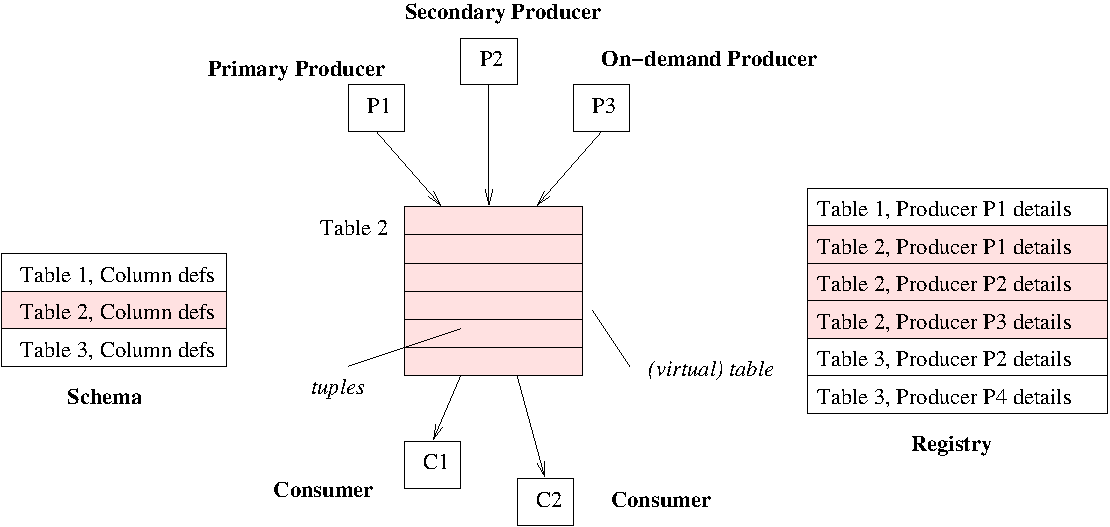
\includegraphics[width=155mm]{virtual_db}
\end{center}

R-GMA presents the data in the form of \emph{virtual databases}, each
containing a set of \emph{virtual tables}. As the picture above shows,
a single\footnote{Although there is only one logical schema and
  registry pair per VDB, replicas are made for scalability and
  robustness. This is discussed in detail later.} schema contains the
name and structure (column names, types and settings) of each virtual
table in the system. A single registry contains a list, for each
table, of producers who have offered to publish rows for the table. A
consumer runs an SQL query against a table, and contacts the registry
to select the best producers to answer the query, contacts each
producer directly, combines the information, and returns a set of
tuples. The mediation process is hidden from the user. Note that there
is no central repository holding the contents of the virtual table; it
is in this sense, that the database is virtual.

\subsubsection{Producers}
\label{sec:producers}
There are three classes of producer: \emph{Primary}, \emph{Secondary}
and \emph{On-demand}. Each is created by a user application and
returns tuples in response to queries from other user
applications. The main difference is in where the tuples come from.

For a primary producer, user's code periodically inserts tuples which
are then stored internally by the producer service. The producer
answers consumer queries from this storage. The secondary producer
service also answers queries from its internal storage, but it
populates this storage itself by running its own query against the
virtual table; the user code only sets the process running; the tuples
come from other producers. In the on-demand producer, there is no
internal storage; data is provided by the user code in direct response
to a query forwarded on to it by the producer service. Examples of the
use of the on-demand producer are not currently included in this
document.

Producers may be set up to use either database or memory storage, with
the data being held in one or two \textit{tuple stores}. One store is
used to answer latest queries. The other store is used for both
history and continuous queries. If no logical name is specified the
data are transient and are removed when the producer is closed down
{--} even if a database is being used to implement the tuple store.

In the case of data base storage, the data can be made persistent by
specifying a logical name for the tuple store. A tuple store is
identified by the logical name and the DN of the user so several
people can use the same logical name. When a producer using a named
tuple store closes down, the tuple store and the data in it are
preserved. When a new producer is created by that user, specifying the
same logical name the tuple store is reused.

The mapping of table names to tables inside the database is carried
out by R{}-GMA and is hidden from the normal user. For those cases
where direct access to the database is needed, a facility is provided
to the sysadmin to determine the mappings from table name to internal
table name for a specified logical name of a tuple store and DN, see
Section \ref{sec:dbMapping}.

Each virtual table has a \emph{key} column (or group of columns)
declared in the schema. Each tuple also carries a \emph{time-stamp},
added by the primary producer when the tuple is first published into
the system, which, together with the key columns, is similar to a
primary key for the table. Tuples with the same key, but different
values for the time-stamp, can also be thought of as different
versions of the same tuple. R-GMA works consistently in
UTC\footnote{UTC refers to Coordinated Universal Time, which used to
  be known as GMT.}. Though the primary producer will add the
time-stamp for you, you can set the date and time yourself. This is
useful if you want to publish some information from a log file for
example. Simply include the \emph{RgmaTimestamp} field in your insert
call. The format is the usual ``YYYY-MM-DDz hh:mm:ss[.s]'' for the
time-stamp.

\subsubsection{Consumers}
\label{sec:consumers}
Each consumer represents a single SQL SELECT query on the virtual
database. The request is initiated by user code, but the
\emph{Consumer Service} carries out all of the work on its behalf. The
query is first passed to the registry to identify which producers, for
each virtual table in the query, must be contacted to answer it. This
process is called \emph{mediation}. The query is then passed by the
consumer service to each relevant producer, to obtain the answer
tuples directly.

There are four types of query: \emph{continuous}, \emph{latest},
\emph{history} and \emph{static}.  The first three types (continuous,
latest and history) can optionally take a \emph{TimeInterval}
parameter.

A continuous query (which can only act on a single table) causes all
new tuples matching the query to be automatically streamed to the
consumer when they are inserted to the virtual table by a producer.
If a time interval parameter is specified, all existing tuples newer
than (\emph{now} - \emph{TimeInterval}) will additionally be returned
when the query is started.

A latest query is evaluated on that set of tuples, which for each
table and key have the greatest time-stamp value and that have not
exceeded their \emph{Latest Retention Period}. In addition, if a time
interval is specified, only tuples that are newer than (\emph{now} -
\emph{TimeInterval}) will be used. Whether or not you specify a time
interval, the query will never use tuples that have exceeded their
latest retention period. The latest retention period is described in
\ref{sec:rp}.

A history query is evaluated over all available versions of tuples.
The set can also be restricted by specifying a time interval.

A static query is handled by an on-demand producer like a normal
one-off database query. There are no time-stamps or retention periods
associated with static queries.

\subsubsection{Meta-data}
\label{sec:metadata}
There are four meta-data fields associated with every tuple, these
are: \textit{ RgmaTimestamp}, \textit{RgmaLRT},
\textit{RgmaOriginalServer} and \textit{RgmaOriginalClient}.

As mentioned above the RgmaTimestamp is normally set by the system to
be the time-stamp when the tuple as inserted into R-GMA. If a value is
set by the user when INSERTing a tuple into a primary producer this
value will be used.

The RgmaLRT holds the \textit{Latest Retention Time.} This field is
user readable but not writable. It is derived by adding the
RgmaTimestamp to the latest retention period associated with the
insert operation. A latest query will never return tuples that have
exceeded the RgmaLRT value.

The RgmaOriginalServer is the name of the server where the data were
inserted if it can be found in the DNS by reverse look-up. Otherwise
it will be a string representation of the numeric IP address.

Finally the RgmaOriginalClient is the name of the user's client
machine that communicated with the RgmaOriginalServer to insert the
data.

None of the meta-data fields are ever modified once the data are
stored.

\subsubsection{Retention Periods}
\label{sec:rp}
To allow primary and secondary producers to periodically purge ``old''
tuples, and to give a precise meaning to the ``current state'' for a
latest query, \emph{retention periods} are used.

The \emph{Latest Retention Period} defines how old a tuple can be
before it should no longer be considered to be the latest. This time
interval is added to the time-stamp and inserted into each tuple
published by a primary producer (RgmaLRT), and remains there when a
tuple is re-published by a secondary producer. In addition, primary
and secondary producers declare a \emph{History Retention Period} for
each table to which they are publishing tuples.

Primary and secondary producers have two logical tuple-stores, one
supporting latest-queries and the other supporting continuous and
history queries. Producers undertake to retain the \emph{most recent}
version of any tuple which has not exceeded its latest retention
period, and \emph{all} versions of any tuple which have not exceeded
the history retention period.

The history retention period may be longer or shorter than the latest
retention period. The history retention period is a (per-table)
property of the producer, whereas the latest retention period is a
property of the tuple.

\subsubsection{Resource Framework and the Termination Interval}
\label{sec:ti}
Each instance of a producer or consumer in a running R-GMA system
exists as a \emph{resource} on a server. Resources have a termination
interval associated with them. The value of the termination
interval is determined by the server but may be queried by the user.

If resource has not been contacted for a period exceeding its
termination interval then the service will close it. This is part of
the soft-state registration process used to ensure that non-existent
resources are removed within a reasonable length of time. A resource
will also be destroyed if the server is restarted. If a user makes a
call via the API after the resource has been closed by the service,
then the system will automatically create a new resource.

A side effect of the system automatically re-creating a consumer
resource is that the query has to be restarted; this may result in
duplicate data being returned. If a query is restarted in this manner
then a warning will be included in the returned tuple set, see Section
\ref{sec:exceptions}.

The user should close a resource manually when it is no longer needed
to conserve resources on the server.
